\documentclass[]{book}

%These tell TeX which packages to use.
\usepackage{array,epsfig}
\usepackage{amsmath}
\usepackage{amsfonts}
\usepackage{amssymb}
\usepackage{amsxtra}
\usepackage{amsthm}
\usepackage{mathrsfs}
\usepackage{color}
\usepackage{graphicx}
\usepackage{bm}
\usepackage{tikz}
\usepackage{float}
\usepackage{titlesec}

\setcounter{secnumdepth}{4}
%\usepackage{widthof}
\usetikzlibrary{arrows}

%Here I define some theorem styles and shortcut commands for symbols I use often
\theoremstyle{definition}
\newtheorem{defn}{Definition}
\newtheorem{thm}{Theorem}
\newtheorem{cor}{Corollary}
\newtheorem*{rmk}{Remark}
\newtheorem{lem}{Lemma}
\newtheorem*{joke}{Joke}
\newtheorem{ex}{Example}
\newtheorem*{soln}{Solution}
\newtheorem{prop}{Proposition}

\newcommand{\lra}{\longrightarrow}
\newcommand{\ra}{\rightarrow}
\newcommand{\surj}{\twoheadrightarrow}
\newcommand{\graph}{\mathrm{graph}}
\newcommand{\bb}[1]{\mathbb{#1}}
\newcommand{\Z}{\bb{Z}}
\newcommand{\Q}{\bb{Q}}
\newcommand{\R}{\bb{R}}
\newcommand{\C}{\bb{C}}
\newcommand{\N}{\bb{N}}
\newcommand{\M}{\mathbf{M}}
\newcommand{\m}{\mathbf{m}}
\newcommand{\MM}{\mathscr{M}}
\newcommand{\HH}{\mathscr{H}}
\newcommand{\Om}{\Omega}
\newcommand{\Ho}{\in\HH(\Om)}
\newcommand{\bd}{\partial}
\newcommand{\del}{\partial}
\newcommand{\bardel}{\overline\partial}
\newcommand{\textdf}[1]{\textbf{\textsf{#1}}\index{#1}}
\newcommand{\img}{\mathrm{img}}
\newcommand{\ip}[2]{\left\langle{#1},{#2}\right\rangle}
\newcommand{\inter}[1]{\mathrm{int}{#1}}
\newcommand{\exter}[1]{\mathrm{ext}{#1}}
\newcommand{\cl}[1]{\mathrm{cl}{#1}}
\newcommand{\ds}{\displaystyle}
\newcommand{\vol}{\mathrm{vol}}
\newcommand{\cnt}{\mathrm{ct}}
\newcommand{\osc}{\mathrm{osc}}
\newcommand{\LL}{\mathbf{L}}
\newcommand{\x}{\bm{x}}
\newcommand{\UU}{\mathbf{U}}
\newcommand{\support}{\mathrm{support}}
\newcommand{\AND}{\;\wedge\;}
\newcommand{\OR}{\;\vee\;}
\newcommand{\Oset}{\varnothing}
\newcommand{\st}{\ni}
\newcommand{\wh}{\widehat}

%Pagination stuff.
\setlength{\topmargin}{-.3 in}
\setlength{\oddsidemargin}{0in}
\setlength{\evensidemargin}{0in}
\setlength{\textheight}{9.in}
\setlength{\textwidth}{6.5in}
\pagestyle{empty}
\renewcommand{\thesection}{\arabic{section}}



\begin{document}

\begin{center}
{\Large Draft}\\
\textbf{Alireza Abrehforoush}\\ %You should put your name here
%Date: 7-27-2022 %You should write the date here.
\end{center}
\vspace{0.2 cm}


\section{Part 1 (2nd\hspace{0.1cm} approach)}
\subsection{Model}
We model the problem with three systems $0$, $1$ and $2$ corresponding to the following set of states of $\left\{ n \right\}$, $\left\{0, n-2\right\}$ and $\left\{1,2,3,\hdots,n-3\right\}$ of previous model respectively. We denote the upper bound of stay of our random walker on expectation in system $i$ by $T_{i}$. 

%graph
\begin{center}
\begin{tikzpicture}
\tikzset{vertex/.style = {shape=circle,draw,minimum size=3em}}
\tikzset{edge/.style = {->,> = latex'}}
% vertices
\node[vertex] (a) at  (0,1.5) {$0^{\prime}$};
\node[vertex] (b) at  (0,0) {$1^{\prime}$};
\node[vertex] (c) at  (0,-1.5) {$2^{\prime}$};
%edges
\draw[->] (a) edge  [loop above] node {$1$} ();
\draw[->] (b) edge  [loop right] node {$1-3p$} ();

\path[->] (b) edge
node[right]{$p$} (a);
\path[->] (b) edge[bend right]      node[left]{$2p$} (c);
\path[->] (c) edge[bend right]      node[right]{$q$} (b);

\draw[->] (c) edge  [loop below] node {$1-q$} ();

\end{tikzpicture}
\end{center}
%graph

We compute an upper bound for expected equilibrium time starting from any arbitrary system ($T$).

\begin{equation}\label{}
\begin{split}
    T &= p\times \left(T_{2} + 2\right) \\
      &+ p\times \left(2T_{2} + 4\right)\times 2p \\
      &+ p\times \left(3T_{2} + 6\right)\times \left(2p\right)^2 \\
      & \vdots \\
      &= \frac{1}{2p} \sum_{i=1}^{\infty} p i \left(T_{2} + 2\right)\left(2p\right)^i \\
      &= \frac{p\left(T_{2} + 2\right)}{\left(1-2p\right)^2}
\end{split}
\end{equation}

To calculate the value of $T_2$ we can use the settings that we had in the first approach.

%graph
\begin{center}
\begin{tikzpicture}
\tikzset{vertex/.style = {shape=circle,draw,minimum size=3em}}
\tikzset{edge/.style = {->,> = latex'}}
% vertices
\node[vertex] (a) at  (-6,0) {$0$};
\node[vertex] (b) at  (-2,0) {$1$};
\node[vertex] (c) at  (2,0) {$2$};
\node[vertex] (d) at  (6,0) {$n-2$};
%edges

\path[->] (a) edge[bend right]
node[below]{$2p$} (b);
\path[->] (b) edge[bend right]
node[above]{$2p$} (a);

\draw[->] (b) edge  [loop above] node {$1-4p$} ();

\path[->] (b) edge[bend right]      node[below]{$2p$} (c);
\path[->] (c) edge[bend right]      node[above]{$2p$} (b);

\draw[->] (c) edge  [loop above] node {$1-4p$} ();

\path (c) to node {\dots} (d);

\end{tikzpicture}
\end{center}
%graph

We consider states $1,2,\ldots,n-3$ corresponding to the configuration with $c = i \in \left\{0,1,\ldots,n\right\}$. 
Let $t_c$ denote the expected reaching time to state $0$ or $n-2$, starting from state $c$.
The changes in $c$ are governed by the following non-homogeneous linear recurrence relation
\begin{equation}    \label{mainEquation}
    t_c 
    = 2p t_{c-1}  + 2p t_{c+1} + (1 - 4p)t_{c} + 1\\
    = \frac{1}{2}t_{c-1} + \frac{1}{2}t_{c+1} + \frac{1}{4p}, \quad c = 1,\ldots,n-3,
\end{equation}
and following initial conditions
\begin{equation}\label{recursiveEquation_t_0}
    t_0 = 0 \qquad t_{n-2} = 0
\end{equation}

We solve the recurrence same way as the first approach. thus, the final closed form is:
\begin{equation} \label{closed form}
    t_c = \frac{c(n-c-2)}{4p}\\
\end{equation}

For every $c \in \left\{0, 1, 2, 3, \hdots, n-2\right\}$ we have:
\begin{equation*} \label{}
    t_c \le t_{\frac{n-2}{2}}
\end{equation*}
So
\begin{equation} \label{}
    T_2 = t_{\frac{n-2}{2}}
\end{equation}

By (1) and (5) we can infer that the expected equilibrium time would be at most 
\begin{equation}\label{}
\begin{split}
    \frac{p\left( \frac{\left(n-2\right)^2}{16p} + 2\right)}{\left(1-2p\right)^2}
\end{split}
\end{equation}
%%%%%%%%%%%%%%%%%%%%%%%%%%%%%%%%%%%%%%%%%%
\section{Extending 2nd approach to m systems}
\begin{figure}[ht]
    \centering
    \includegraphics[width=0.4\textwidth]{figures/3.jpg}
    \caption{configuration with 3 red arcs of length one, two and three}
    \label{fig:mesh1}
\end{figure}
For each set of configurations with same number of arcs, we consider a unique system that includes all these configurations. we denote the upper bound of stay of our random walker in system $i$ by \emph{$T_i$}. also \emph{$p_{i, j}$} denotes the probability of reaching from system $i$ to system $j$ in one step. and finally, \emph{$t_{i, j}$} denotes the reaching time to system $j$ for the first time, starting from system $i$.
%graph
\begin{center}
\begin{tikzpicture}
\tikzset{vertex/.style = {shape=circle,draw,minimum size=3em}}
\tikzset{edge/.style = {->,> = latex'}}
% vertices
\node[vertex] (a) at  (-6,0) {$0^{\prime}$};
\node[vertex] (b) at  (-2,0) {$1^{\prime}$};
\node[vertex] (c) at  (2,0) {$2^{\prime}$};
\node[vertex] (d) at  (6,0) {$\left\lfloor \frac{n}{2} \right\rfloor ^{\prime}$};
%edges

\path[->] (a) edge[bend left]
node[above]{$p_{0,1}$} (b);
\path[->] (b) edge[bend left]
node[below]{$p_{1,0}$} (a);
\path[->] (b) edge[bend left]
node[above]{$p_{1,2}$} (c);
\path[->] (c) edge[bend left]
node[below]{$p_{2,1}$} (b);
\path (c) to node {\dots} (d);


\end{tikzpicture}
\end{center}
%graph

 We may have following recurrence relation for $t$s:
\begin{equation}
\begin{split}
    t_{c, 0} = t_{c, c-1} + t_{c-1, c-2} + \hdots + t_{1, 0}
\end{split}
\end{equation}

\begin{equation}
\begin{split}
    t_{c, c-1} = p_{c, c+1} t_{c+1, c-1} + \left( 1 - p_{c, c+1} - p_{c, c-1} \right) t_{c, c-1} + p_{c, c-1} + 1
\end{split}
\end{equation}


%%%%%%%%%%%%%%%%%%%%%%%%%%%%%%%%%%%%%%%%%%
\section{New approach for main problem (asynchronous version) (probably similar to the phase transition paper)}
\subsection{Model}
For any configuration \emph{$c$} with $n$ agents there exists a string of $0$s and $1$s with length $n$, each $0$s and $1$s corresponding to black arc (equilibrium) and red arc (not equilibrium) respectively.
the activation of any agent between arcs $i$ and $i+1$ leads to one of the following modifications in the string:
\begin{center}
    \begin{table}[ht]
        \begin{tabular}{|l|l|}
        \hline
        00 & 11 \\ \hline
        01 & 10 \\ \hline
        10 & 01 \\ \hline
        11 & 11 \\ \hline
        \end{tabular}
    \end{table}
\end{center}

We denote the number of red arcs in configuration $c$ by $r(c)$. also we denote configuration in next step (current configuration is $c$) by $\delta(c)$.
We denote the $r(\delta(c)) - r(c)$ by $\Delta r$ and compute its expected value as follows:

\begin{equation}
\begin{split}
    \mathbb{E}[\Delta r] &= \mathbb{E}[\Delta r | \text{activation of agent between two red arcs}] \times \mathbb{P}\left\{ \text{activation of agent between two red arcs} \right\} \\
    &+ \mathbb{E}[\Delta r | \text{activation of agent not between two red arcs}] \times \mathbb{P}\left\{ \text{activation of agent not between two red arcs} \right\} \\
    &= -2\times \mathbb{P}\left\{ \text{activation of agent between two red arcs} \right\}
\end{split}
\end{equation}
If we have such a lower bound for $\mathbb{P}\left\{ \text{activation of agent between two red arcs} \right\}$ in any configuration, we can calculate an upper bound for the expected time of reaching to equilibrium through dividing number of red arcs by $\mathbb{E}[\Delta r]$. (failed. because it can be zero :( )

\newpage
\vspace{0.2 cm}
%%%%%%%%%%%%%%%%%%%%%%%%%%%%%%%%%%%%%%%%%%%
\section{Configurations with more than two red arcs of length one (asynchronous)}
\begin{figure}[H]
    \centering
    \includegraphics[width=0.4\textwidth]{figures/pic2.jpg}
    \caption{configuration with $\left(c_{1}, c_{2}, c_{3}, c_{4}, c_{5}, c_{6}\right) = \left(5, 4, 0, 3, 0, 0\right)$}
    \label{fig:mesh2}
\end{figure}
Corresponding to all configurations with $i$ red arcs of length one (for simplicity from now on we call it red arcs), we consider a \emph{system} $i^\prime$ in which our random walker is wandering and leaves it after a while. as in asynchronous dynamics the number of red arcs is descending and at each time at most two red arcs can disappear (by activation of the agent adjacent to two red arcs), these systems can be modeled through below directed path graphs regarding the parity of number of red arcs of length one at the beginning ($m$):

%graph
\begin{figure}[H]
    \centering
    \begin{tikzpicture}
    \tikzset{vertex/.style = {shape=circle,draw,minimum size=3em}}
    \tikzset{edge/.style = {->,> = latex'}}
    % vertices
    \node[vertex] (a) at  (-6,0) {$0^\prime$};
    \node[vertex] (b) at  (-2,0) {$2^\prime$};
    \node[vertex] (c) at  (2,0) {$4^\prime$};
    \node[vertex] (d) at  (6,0) {$m^\prime$};
    %edges
    \path[->] (b) edge
    node[above]{} (a);
    \path[->] (c) edge
    node[above]{} (b);
    
    \path (c) to node {\dots} (d);
    \end{tikzpicture}
    \caption{systems starting with at most even number of red arcs of length one ($m$)}
\end{figure}
%graph
%graph
\begin{figure}[H]
    \centering
    \begin{tikzpicture}
    \tikzset{vertex/.style = {shape=circle,draw,minimum size=3em}}
    \tikzset{edge/.style = {->,> = latex'}}
    % vertices
    \node[vertex] (a) at  (-6,0) {$1^\prime$};
    \node[vertex] (b) at  (-2,0) {$3^\prime$};
    \node[vertex] (c) at  (2,0) {$5^\prime$};
    \node[vertex] (d) at  (6,0) {$m^\prime$};
    %edges
    \path[->] (b) edge
    node[above]{} (a);
    \path[->] (c) edge
    node[above]{} (b);
    
    \path (c) to node {\dots} (d);
    \end{tikzpicture}
    \caption{systems starting with at most odd number of red arcs of length one ($m$)}
\end{figure}
%graph

We denote the upper bound of stay time of our random walker on expectation in system $i$ by $T_{i}$. so the expected time to reach equilibrium starting from any arbitrary configuration ($T$) is the expected time of reaching from system $m^\prime$ to system $0^\prime$:

\begin{equation}
    T = \sum_{i = 0}^{m} T_i
\end{equation}

For computing $T$ we have two following approaches:
\subsection{Using  part 1}

$X$ and $Y$ (red arcs in below figure) are the first two red arcs that disappear in this configuration (Obviously $X$ and $Y$ are two adjacent red arcs). Thus we ignore other unstable arcs (shown with pink).

\begin{figure}[ht]
    \centering
    \includegraphics[width=0.4\textwidth]{figures/m.arcs.jpg}
    \caption{}
    \label{fig:mesh3}
\end{figure}


We can model problem through following Markov chain. Assuming $X$ and $Y$ are the first two red arcs that disappear, state $i$ corresponds to the configuration in which $i$ black arcs exist between $X$ and $Y$. So the probability of reaching to system $(m-2)^\prime$ through states $1$ to $n-m$ in one step is zero.

%graph
\begin{figure}[H]
    \centering
    \begin{tikzpicture}
    \tikzset{vertex/.style = {shape=circle,draw,minimum size=3em}}
    \tikzset{edge/.style = {->,> = latex'}}
    % vertices
    \node[vertex] (b) at  (-3,3) {$n-m+1$};
    \node[vertex] (b2) at  (0,3) {$n-m+2$};
    \node[vertex] (b3) at  (5,3) {$n-1$};
    
    \node[vertex] (a) at  (-4,0) {$0$};
    \node[vertex] (c) at  (6,0) {$n-m$};
    \node[vertex] (d) at  (1,-3) {$(m-2)^\prime$};
    \node[vertex] (a1) at (-2,0) {$1$};
    \node[vertex] (a2) at (0,0) {$2$};
    %edges
    \draw[->] (a) edge  [loop above] node {$1-3p$} ();
    \draw[->] (b) edge  [loop above] node {$1$} ();
    \draw[->] (b2) edge  [loop above] node {$1$} ();
    \draw[->] (b3) edge  [loop above] node {$1$} ();
    \draw[->] (c) edge  [loop above] node {$1-2p$} ();
    \draw[->] (a1) edge  [loop above] node {$1-4p$} ();
    \draw[->] (a2) edge  [loop above] node {$1-4p$} ();
    
    \path[->] (a) edge[bend right]      node[above]{$p$} (d);
    
    \path[->] (a) edge[bend left]     node[above]                      {2p} (a1);
    \path[->] (a1) edge[bend left]     node[above]                      {2p} (a);
    
    \path[->] (a1) edge[bend left]     node[above]                      {2p} (a2);
    \path[->] (a2) edge[bend left]     node[above]                      {2p} (a1);

    %
    \path (b2) to node {\dots} (b3);
    %
    
    \path (a2) to node {\dots} (c);
    \node [shape=circle,minimum size=1.5em] (a3) at (2,0) {};
    \path[->] (a2) edge[bend left]     node[above]                      {2p} (a3);
    \path[->] (a3) edge[bend left]     node[above]                      {2p} (a2);
    
    \node [shape=circle,minimum size=1.5em] (c1) at (4,0) {};
    \path[->] (c) edge[bend left]     node[above]                      {2p} (c1);
    \path[->] (c1) edge[bend left]     node[above]                      {2p} (c);
    \end{tikzpicture}
    \caption{system with $m$ red arcs}
\end{figure}
%graph

We consider states $0, 1, \hdots, n$ corresponding to the configurations with $c = i \in \{0, 1, . . . , n\}$. Let $t_c$ denote the expected transition time from system $m^\prime$ to $(m-2)^\prime$, starting from state $c$. The changes in $c$ are governed by the following recursive equation:
\begin{equation}
    t_c 
    = 2p t_{c-1}  + 2p t_{c+1} + (1 - 4p)t_{c} + 1\\
    = \frac{1}{2}t_{c-1} + \frac{1}{2}t_{c+1} + \frac{1}{4p}, \qquad c = 1,\ldots,n-m-1,
\end{equation}
with following initial conditions:
\begin{equation}
\begin{split}
    &t_0 = p\times 0 + 2pt_1 + (1-3p)t_0  + 1 = \frac{2}{3}t_1 + \frac{1}{3p} \\
    &t_{n-m} = 2pt_{n-m-1} + \left( 1-2p \right)t_{n-m} = t_{n-m-1} + \frac{1}{2p}
\end{split}
\end{equation}
From (2) and (3) we can infer
\begin{multline*}
    \\
    t_1 = \frac{1}{2}t_0 + \frac{1}{2}t_2 + \frac{1}{4p}\\
    t_2 = \frac{1}{2}t_1 + \frac{1}{2}t_3 + \frac{1}{4p}\\
    t_3 = \frac{1}{2}t_2 + \frac{1}{2}t_4 + \frac{1}{4p}\\
    \vdots\\
    t_{n-m-1} = \frac{1}{2}t_{n-m-2} + \frac{1}{2}t_{n-m} + \frac{1}{4p}\\
    \sum_{i=1}^{n-m-1} t_i = \frac{1}{2}\left[ \sum_{i=0}^{n-m-2} t_i + \sum_{i=2}^{n-m} t_i \right] + \frac{n-m-1}{4p} \Rightarrow t_1 + t_{n-m-1} = \frac{1}{2}\left(t_0 + t_1 + t_{n-m-1} + t_{n-m}\right) + \frac{n-m-1}{4p}\\
    \Rightarrow t_1 + t_{n-m-1} = t_0 + t_{n-m} + \frac{n-m-1}{2p}
\end{multline*}

Using (3) we can infer

\begin{center}
\begin{equation}
    t_1 = \frac{2}{3}t_1 + \frac{1}{3p} + \frac{1}{2p} + \frac{n-m-1}{2p} \Rightarrow t_1 = \frac{3n-3m+2}{2p}
\end{equation}
\begin{equation}
    t_0 = \frac{2}{3}t_1 + \frac{1}{3p} = \frac{n-m+1}{p}
\end{equation}
\end{center}

We now have a non-homogeneous linear recurrence relation with (2) as relation and (4) and (5) as initial conditions. The solution ($t_c$)
of a non-homogeneous recurrence relation has two parts.
First part is the solution ($t^{(h)}_{c}$)
of the associated homogeneous recurrence relation and the second part is the particular solution ($t^{(p)}_{c}$).
$$
        t_c = t^{(h)}_{c} + t^{(p)}_{c}
$$
First we rewrite (2) in standard form.
\begin{equation}
    t_{c+1} = 2t_c - t_{c-1} - \frac{1}{2p}
\end{equation}
The characteristic polynomial corresponding to the homogeneous part is as follows:
$$
r^2 - 2r + 1 = 0 \Rightarrow r = 1
$$
Thus the general solution is of the form
$$
t_c = \alpha_{1}c 1^c + \alpha_{2} 1^c
$$
Armed with that knowledge, and since the non-homogeneous part is also a polynomial (in this case of degree zero) which is itself a degenerate case of being of the form $1^c$ as well, we multiply by $c$ enough times to make it distinct from the other already known parts. I.e. we expect the non-homogeneous part to be of the form $\beta c^2$. Plugging this into the recurrence, we have:
$$
\beta (c+1)^2 = 2\beta c^2 - \beta (c-1)^2 - \frac{1}{2p} \Rightarrow \beta = -\frac{1}{4p}
$$
So, we expect
$$
t_c = \alpha_1 c + \alpha_2 - \beta c^2 = \alpha_1 c + \alpha_2 -\frac{1}{4p}c^2
$$
using initial conditions we have:
$$
t_0 = \alpha_1 \times 0 + \alpha_2 - \frac{1}{4p}\times 0 = \frac{n-m+1}{p} \\
\Rightarrow \alpha_2 = \frac{n-m+1}{p}
$$
and
$$
t_1 = \alpha_1 + \frac{n-m+1}{p} -\frac{1}{4p} = \frac{3n-3m+2}{2p} \Rightarrow \alpha_1 = \frac{2n-2m+1}{4p}
$$
Thus, the final closed form is:
\begin{equation}
    t_c = \frac{(c+2)(2n-2m) - c^2 + c + 4}{4p}\\
    \qedsymbol
\end{equation}
From (1) and the fact that the number of red arcs can not be more than $n$, the upper bound for expected equilibrium time is $O(n^3)$.

\subsection{Using recurrence relation}
Consider a configuration with $m$ red arcs which the distance between each two of them is an integer from the set $\left\{ 0,1,2,\hdots,n-1 \right\}$. We can denote this configuration by $\left( c_{1}, c_{2}, \hdots, c_{m} \right)$ (and any circular shift of the distances). Let $t_{c_{1},c_{2},\hdots,c_{m}}$ denote the expected equilibrium time, starting from state $\left( c_{1}, c_{2}, \hdots, c_{m} \right)$. The changes in $\left( c_{1}, c_{2}, \hdots, c_{m} \right)$ in any arbitrary configuration are governed by the following recursive
equation:
\begin{equation}
\begin{split}
    \forall i: c_i \neq 0 \qquad
    t_{c_1, c_2, \hdots, c_m} &= \sum_{i = 1}^{m} pt_{c_1, \hdots, c_{i}-1, c_{i+1}+1, \hdots, c_m} + pt_{c_1, \hdots, c_{i-1}+1, c_{i}-1, \hdots, c_m} \\
    &+ \left(1 - 2mp\right)\left( t_{c_{1}, c_{2}, \hdots, c_{m}} \right) \\
    &+ 1
\end{split}
\end{equation}
and following initial conditions (every configuration with at least one black arc of length 0):
\begin{equation}
\begin{split}
    \chi = \left\{ i:c_i = 0 \right\} \qquad t_{c_1, c_2, \hdots, c_m} &= \sum_{i \notin \chi} pt_{c_1, \hdots, c_{i}-1, c_{i+1}+1, \hdots, c_m} + pt_{c_1, \hdots, c_{i-1}+1, c_{i}-1, \hdots, c_m} \\
    &+ \sum_{i \in \chi} pt_{c_1, \hdots, c_{i-2}, c_{i-1} + 2 + c_{i+1}, c_{i+2}, \hdots, c_m} \\
    &+ \left( 1 - |\chi| - 2|\chi^\prime| \right)pt_{c_1, c_2, \hdots, c_m} \\
    &+ 1
\end{split}
\end{equation}


\newpage
\vspace{0.2 cm}
%%%%%%%%%%%%%%%%%%%%%%%%%%%%%%%%%%%%%%%%%%%
\section{Synchronous dynamics}
\begin{figure}[H]
    \centering\includegraphics[width=0.4\textwidth]{figures/pic2.jpg}
    \caption{configuration with $\left(c_{1}, c_{2}, c_{3}, c_{4}, c_{5}, c_{6}\right) = \left(5, 4, 0, 3, 0, 0\right)$}
    %\label{fig:mesh2}
\end{figure}
\begin{figure}[H]
    \centering
    \includegraphics[width=0.4\textwidth]{figures/sync.jpg}
    \caption{configuration with $\left(c_{1}, c_{2}, c_{3}, c_{4}, c_{5}, c_{6}, c_{7}, c_{8}, c_{9}, c_{10}\right) = \left(1, 0, 2, 0, 2, 2, 0, 0, 0, 0\right)$}
    %\label{fig:mesh2}
\end{figure}

Corresponding to all configurations with $i$ red arcs of length one (for simplicity from now on we call it red arcs), we consider a \emph{system} $i^\prime$ in which our random walker is wandering and leaves it after a while. As in synchronous dynamics at each time step, the number of red arcs is either ascending (appearance of red arcs due to activation of all coordinating agents on an arc by at most twice number of current red arcs) or descending (disappearance of any number of red arcs due to activation of the agent adjacent to two red arcs), these systems can be modeled through below directed graphs regarding the parity of number of red arcs of length one at the beginning ($m$):

%graph
\begin{figure}[H]
    \centering
    \begin{tikzpicture}
    \tikzset{vertex/.style = {shape=circle,draw,minimum size=3em}}
    \tikzset{edge/.style = {->,> = latex'}}
    % vertices
    \node[vertex] (a0) at  (0,0) {$0^\prime$};
    
    \node[vertex] (a2) at  (0,-2) {$2^\prime$};
    \node[vertex] (b0) at  (-2,-4) {$0^\prime$};
    \node[vertex] (b4) at  (0,-4) {$4^\prime$};
    \node[vertex] (b6) at  (2,-4) {$6^\prime$};
    \path[->] (a2) edge
    node[above]{} (b0);
    \path[->] (a2) edge
    node[above]{} (b4);
    \path[->] (a2) edge
    node[above]{} (b6);
%%%%%%%%%%%%%%%%%
    \node[vertex] (a4) at  (0,-6) {$4^\prime$};
    \node[vertex] (c0) at  (-5,-8) {$0^\prime$};
    \node[vertex] (c2) at  (-3,-8) {$2^\prime$};
    \node[vertex] (c6) at  (-1,-8) {$6^\prime$};
    \node[vertex] (c8) at  (1,-8) {$8^\prime$};
    \node[vertex] (c10) at  (3,-8) {$10^\prime$};
    \node[vertex] (c12) at  (5,-8) {$12^\prime$};
    \path[->] (a4) edge
    node[above]{} (c0);
    \path[->] (a4) edge
    node[above]{} (c2);
    \path[->] (a4) edge
    node[above]{} (c6);
    \path[->] (a4) edge
    node[above]{} (c8);
    \path[->] (a4) edge
    node[above]{} (c10);
    \path[->] (a4) edge
    node[above]{} (c12);
%%%%%%%%%%%%%%%%%
    \node[vertex] (a6) at  (0,-10) {$6^\prime$};
    \node[vertex] (d0) at  (-8,-12) {$0^\prime$};
    \node[vertex] (d2) at  (-6,-12) {$2^\prime$};
    \node[vertex] (d4) at  (-4,-12) {$4^\prime$};
    \node[vertex] (d8) at  (-2,-12) {$8^\prime$};
    \node[vertex] (d10) at  (0,-12) {$10^\prime$};
    \node[vertex] (d12) at  (2,-12) {$12^\prime$};
    \node[vertex] (d14) at  (4,-12) {$14^\prime$};
    \node[vertex] (d16) at  (6,-12) {$16^\prime$};
    \node[vertex] (d18) at  (8,-12) {$18^\prime$};
    \path[->] (a6) edge
    node[above]{} (d0);
    \path[->] (a6) edge
    node[above]{} (d2);
    \path[->] (a6) edge
    node[above]{} (d4);
    \path[->] (a6) edge
    node[above]{} (d8);
    \path[->] (a6) edge
    node[above]{} (d10);
    \path[->] (a6) edge
    node[above]{} (d12);
    \path[->] (a6) edge
    node[above]{} (d14);
    \path[->] (a6) edge
    node[above]{} (d16);
    \path[->] (a6) edge
    node[above]{} (d18);
%%%%%%%%%%%%%%%%%
    \node[vertex] (a) at  (0,-16) {$n^\prime$};
    \node[vertex] (e0) at  (-6,-18) {$0^\prime$};
    \node[vertex] (e2) at  (-4,-18) {$2^\prime$};
    \node[vertex] (en_2) at  (6,-18) {$(n-2)^\prime$};
    \path[->] (a) edge
    node[above]{} (e0);
    \path[->] (a) edge
    node[above]{} (e2);
    \path[->] (a) edge
    node[above]{} (en_2);
    \path (e2) to node {\dots} (en_2);
    
    
    \path (d10) to node {\vdots} (a);

    \end{tikzpicture}
    \caption{systems starting with at most even number of red arcs of length one ($m$)}
\end{figure}
%graph
and respectively for odd number of red arcs.

We denote the upper bound of stay time of our random walker on expectation in system $i$ and reaching to system $j$ by $T_{i, j}$. So the expected time to reach equilibrium starting from any arbitrary configuration ($T$) would be sum of $T_{i,j}$s.



For computing $T$ we have two following approaches:
\subsection{Using  part 1}

We assume $X_1, X_2, \hdots, X_k$ are the red arcs that disappear in this configuration in next time step (Obviously $X$s must be adjacent pairwise) and $Y_1, Y_2, \hdots, Y_h$  are black arcs that appear in this configuration in next time step (Obviously $Y$s must be the black arcs adjacent to ending red arcs of a consecutive adjacent red arcs)


\subsection{Using recurrence relation}

%%%%%%%%%%%%%%%%%%%%%%%%%%%%%%%%%%%%%%%%%%%
%%%%%%%%%%%%%%%%%%%%%%%%%%%%%%%%%%%%%%%%%%%
%%%%%%%%%%%%%%%%%%%%%%%%%%%%%%%%%%%%%%%%%%%
%%%%%%%%%%%%%%%%%%%%%%%%%%%%%%%%%%%%%%%%%%%
%%%%%%%%%%%%%%%%%%%%%%%%%%%%%%%%%%%%%%%%%%%
%%%%%%%%%%%%%%%%%%%%%%%%%%%%%%%%%%%%%%%%%%%
%%%%%%%%%%%%%%%%%%%%%%%%%%%%%%%%%%%%%%%%%%%
%%%%%%%%%%%%%%%%%%%%%%%%%%%%%%%%%%%%%%%%%%%
\newpage

\subsection{Pure decrease of red arcs}
\subsubsection{for $n = 6$}
\begin{figure}[H]
    \centering
    \includegraphics[width=0.4\textwidth]{figures/n60.jpg}
    \caption{}
\end{figure}
\begin{equation}
\begin{split}
    t_0 &= \left[ p \left( 1-p \right)^2 \right] \times 0 \\
    &+ \left[ 1 - 3p\left( 1-p \right)^2 - p^2\left( 1-p\right) \right] \times t_0 \\
    &+ \left[ 2p\left( 1-p \right)^2 \right] \times t_1 \\
    &+ \left[ p^2 \left( 1-p \right) \right] \times t_2 \\
    &+ 1
\end{split}
\end{equation}


\begin{figure}[H]
    \centering
    \includegraphics[width=0.4\textwidth]{figures/n61.jpg}
    \caption{}
\end{figure}
\begin{equation}
\begin{split}
    t_1 &= \left[ p^2 \left( 1-p \right)^2 \right] \times 0 \\
    &+ \left[ 2p\left( 1-p \right)^3 + 2p^3\left( 1-p \right) \right] \times t_0 \\
    &+ \left[ 1 - 4p\left( 1-p \right)^3 - 2p^3\left( 1-p \right) - p^2\left( 1-p \right)^ 2 \right] \times t_1 \\
    &+ \left[ 2p \left( 1-p \right)^3 \right] \times t_2 \\
    &+ 1
\end{split}
\end{equation}


\begin{figure}[H]
    \centering
    \includegraphics[width=0.4\textwidth]{figures/n62.jpg}
    \caption{}
\end{figure}
\begin{equation}
\begin{split}
    t_2 &= \left[ 2p^2 \left( 1-p \right)^2 \right] \times t_0 \\
    &+ \left[ 4p\left( 1-p \right)^3 \right] \times t_1 \\
    &+ \left[ 1 - 4p\left( 1-p \right)^3 - 2p^2\left( 1-p \right)^2 \right] \times t_2 \\
    &+ 1
\end{split}
\end{equation}
We write equations as following matrix operations:
\begin{equation}
\begin{split}
\begin{pmatrix}
3p\left( 1-p \right)^2 + p^2\left( 1-p\right) &        -2p\left( 1-p \right)^2  & -p^2\left( 1-p \right)^2 \\
-2p\left( 1-p \right)^3 - 2p^3\left( 1-p \right) & 4p\left( 1-p \right)^3 + 2p^3\left( 1-p \right) + p^2\left( 1-p \right)^ 2                      &        -2p \left( 1-p \right)^3 \\
-2p^2 \left( 1-p \right)^2                    &        -4p\left( 1-p \right)^3  &  4p\left( 1-p \right)^3 + 2p^2\left( 1-p \right)^2
\end{pmatrix}
\begin{pmatrix}
t_0 \\
t_1 \\
t_2
\end{pmatrix}
=
\begin{pmatrix}
1 \\
1 \\
1
\end{pmatrix}
\end{split}
\end{equation}
And values of $t_i$s is as follows:
\begin{equation}
\begin{split}
t_0 &= \frac{2\,p^4-11\,p^3+35\,p^2-44\,p+20}{2\,p\,{\left(p-1\right)}^3\,\left(p^3-p^2+2\,p-4\right)} \\ \\
t_1 &= \frac{2\,p^4-11\,p^3+29\,p^2-32\,p+13}{p\,{\left(p-1\right)}^3\,\left(p^3-p^2+2\,p-4\right)} \\ \\
t_2 &= \frac{6\,p^4-30\,p^3+67\,p^2-69\,p+28}{2\,p\,{\left(p-1\right)}^3\,\left(p^3-p^2+2\,p-4\right)} \\ \\
t_3 &= t_1 \\ \\
t_4 &= t_0
\end{split}
\end{equation}




\subsubsection{Arbitrary $n$}
\begin{figure}[H]
    \centering
    \includegraphics[width=0.4\textwidth]{figures/sync_pure_increase_2.jpg}
    \caption{}
\end{figure}
First of all we try to calculate the expected time to reach equilibrium from a configuration with two red arcs of length 1 (above figure). The recurrence relation is as follows:
\begin{equation}
\begin{split}
    t_c &= \left[2p\left(1-p\right)^3\right] \times \left( t_{c-1}+t_{c+1} \right) \\
    &+ \left[p^2\left(1-p\right)^2\right] \times \left( t_{c-2}+t_{c+2} \right) \\
    &+ \left[1-4p\left(1-p\right)^3-2p^2\left(1-p\right)^2\right] \times t_c \\
    &+ 1,  \quad c = 2,\ldots,n-4
\end{split}
\end{equation}
with following initial conditions:
\begin{equation}
\begin{split}
    t_0 &= \left[ p^2(1-p) \right] \times t_2 \\
    &+ \left[ 2p(1-p)^2 \right] \times t_1 \\
    &+ \left[ 1 -  p^2(1-p) - 3p(1-p)^2 \right] \times t_0 \\
    &+ 1 \\
\end{split}
\end{equation}

\begin{equation}
\begin{split}
    t_1 &= \left[ p^2(1-p)^2 \right] \times t_3 \\
    +& \left[ 2p(1-p)^3 \right] \times t_2 \\
    +& \left[ 1 - 2p^2(1-p)^2 - 4p(1-p)^3 \right] \times t_1 \\ 
    +& \left[ 2p(1-p)^3 \right] \times t_0 \\
    +& 1 \\
\end{split}
\end{equation}
The equations for $n=10$ is as follows:
\begin{equation}
\begin{split}
2t_2+2t_3=2\beta t_0 + (1-\gamma)t_1 + (1+\gamma)t_2 +
(2-2\beta)t_3 +
t_4 +
5 \\
2\beta
\end{split}
\end{equation}
Solution of $n=10$ is as follows:
\begin{equation}
\begin{split}
    t_0 &= -\frac{2\,p^5+7\,p^4-72\,p^3+44\,p^2+160\,p-144}{16\,p^2\,\left(p^2-2\right)\,{\left(p-1\right)}^3} \\ \\
    t_1 &= -\frac{2\,p-9}{2\,p^2\,{\left(p-1\right)}^2} \\ \\
    t_2 &= -\frac{-2\,p^5+13\,p^4-90\,p^3+84\,p^2+136\,p-144}{16\,p^2\,\left(p^2-2\right)\,{\left(p-1\right)}^3} \\ \\
    t_3 &= -\frac{2\,p^3-25\,p^2+8\,p+36}{4\,p^2\,\left(p^2-2\right)\,{\left(p-1\right)}^2} \\ \\
    t_4 &= -\frac{2\,p^5+7\,p^4-120\,p^3+148\,p^2+104\,p-144}{16\,p^2\,\left(p^2-2\right)\,{\left(p-1\right)}^3} \\ \\
    t_5 &= -\frac{2\,p^3-25\,p^2+8\,p+36}{4\,p^2\,\left(p^2-2\right)\,{\left(p-1\right)}^2} \\ \\
    t_6 &= -\frac{-2\,p^5+13\,p^4-90\,p^3+84\,p^2+136\,p-144}{16\,p^2\,\left(p^2-2\right)\,{\left(p-1\right)}^3} \\ \\
    t_7 &= -\frac{2\,p-9}{2\,p^2\,{\left(p-1\right)}^2} \\ \\
    t_8 &= -\frac{2\,p^5+7\,p^4-72\,p^3+44\,p^2+160\,p-144}{16\,p^2\,\left(p^2-2\right)\,{\left(p-1\right)}^3} \\ \\
\end{split}
\end{equation}
We write equations (1), (2), and (3) as following matrix operation:\\
\setcounter{MaxMatrixCols}{20}
\resizebox{.9\hsize}{!}{$
\begin{bmatrix}
p^2\left( 1-p \right) + 3p\left( 1-p \right)^2 & -2p\left( 1-p \right)^2 & -p^2\left( 1-p \right) & 0 & 0 & 0 & 0 & 0 & 0 & \cdots & 0 \\
0 & 2p^2\left( 1-p \right)^2+4p\left( 1-p \right)^3 & -2p\left( 1-p \right)^3 & -p^2\left( 1-p \right)^2 & 0 & 0 & 0 & 0 & 0 & \cdots & 0 \\
-p^2\left( 1-p \right)^2 & -2p\left( 1-p \right)^3 & 4p\left( 1-p \right)^3+2p^2\left( 1-p \right)^2 & -2p\left( 1-p \right)^3 & -p^2\left( 1-p \right)^2 & 0 & 0 & 0 & 0 & \cdots & 0 \\
0 & -p^2\left( 1-p \right)^2 & -2p\left( 1-p \right)^3 & 4p\left( 1-p \right)^3+2p^2\left( 1-p \right)^2 & -2p\left( 1-p \right)^3 & -p^2\left( 1-p \right)^2 & 0 & 0 & 0 & \cdots & 0 \\
0 & 0 & -p^2\left( 1-p \right)^2 & -2p\left( 1-p \right)^3 & 4p\left( 1-p \right)^3+2p^2\left( 1-p \right)^2 & -2p\left( 1-p \right)^3 & -p^2\left( 1-p \right)^2 & 0 & 0 & \cdots & 0 \\
0 & 0 & 0 & -p^2\left( 1-p \right)^2 & -2p\left( 1-p \right)^3 & 4p\left( 1-p \right)^3+2p^2\left( 1-p \right)^2 & -2p\left( 1-p \right)^3 & -p^2\left( 1-p \right)^2 & 0 & \cdots & 0 \\
\vdots & & & & & & & & & & \\
0 & 0 & 0 & 0 & \cdots & 0 & -p^2\left( 1-p \right)^2 & -2p\left( 1-p \right)^3 & 4p\left( 1-p \right)^3+2p^2\left( 1-p \right)^2 & -2p\left( 1-p \right)^3 & -p^2\left( 1-p \right)^2 \\

0 & \cdots & 0 & 0 & 0 & 0 & 0 & -p^2\left( 1-p \right)^2 & -2p\left( 1-p \right)^3 & 2p^2\left( 1-p \right)^2+4p\left( 1-p \right)^3 & 0 \\

0 & \cdots & 0 & 0 & 0 & 0 & 0 & 0 & -p^2\left( 1-p \right) & -2p\left( 1-p \right)^2 & p^2\left( 1-p \right) + 3p\left( 1-p \right)^2
\end{bmatrix}
\begin{bmatrix}
t_0 \\
 \\
 \\
 \\
\vdots  \\
 \\
 \\
 \\
 \\
t_{n-2}
\end{bmatrix}
=
\begin{bmatrix}
1 \\
 \\
 \\
 \\
\vdots  \\
 \\
 \\
 \\
 \\
1
\end{bmatrix}
$}
we simplify above equations with variables as follows:\\
\setcounter{MaxMatrixCols}{20}
\resizebox{.9\hsize}{!}{$
\begin{bmatrix}
\delta & \epsilon & \varepsilon & 0 & 0 & 0 & 0 & 0 & 0 & \cdots & 0 \\

0 & \zeta & \eta & \theta & 0 & 0 & 0 & 0 & 0 & \cdots & 0 \\

\alpha & \beta & \gamma & \beta & \alpha & 0 & 0 & 0 & 0 & \cdots & 0 \\

0 & \alpha & \beta & \gamma & \beta & \alpha & 0 & 0 & 0 & \cdots & 0 \\

0 & 0 & \alpha & \beta & \gamma & \beta & \alpha & 0 & 0 & \cdots & 0 \\

0 & 0 & 0 & \alpha & \beta & \gamma & \beta & \alpha & 0 & \cdots & 0 \\

\vdots & & & & & & & & & & \\

0 & 0 & 0 & 0 & \cdots & 0 & \alpha & \beta & \gamma & \beta & \alpha \\

0 & \cdots & 0 & 0 & 0 & 0 & 0 & \theta & \eta & \zeta & 0 \\

0 & \cdots & 0 & 0 & 0 & 0 & 0 & 0 & \varepsilon & \epsilon & \delta
\end{bmatrix}
\begin{bmatrix}
t_0 \\
 \\
 \\
 \\
\vdots  \\
 \\
 \\
 \\
 \\
t_{n-2}
\end{bmatrix}
=
\begin{bmatrix}
1 \\
 \\
 \\
 \\
\vdots  \\
 \\
 \\
 \\
 \\
1
\end{bmatrix}
$}

% \begin{equation}
% \begin{split}
% \sum_{i=4}^{n-2}t_i=\frac{2p-2}{p}\sum_{i=3}^{n-3}t_i
% +\frac{4-2p}{p}\sum_{i=2}^{n-4}t_i
% +\frac{2p-2}{p}\sum_{i=1}^{n-5}t_i
% -\sum_{i=0}^{n-6}t_i
% +\frac{-(n-1)}{p^2(1-p)^2} \\
% \Rightarrow
% 2t_0+\frac{4-2p}{p}t_1-\frac{4-2p}{p}t_2-2t_3=\frac{-(n-1)}{p^2(1-p)^2}
% \end{split}
% \end{equation}
% Recurrence relation is standard form:
% \begin{equation}
% \begin{split}
%     t_{c+2} &= \frac{2p-2}{p}t_{c+1} \\
%     +& \frac{4-2p}{p}t_{c} \\
%     +& \frac{2p-2}{p}t_{c-1} \\
%     -& t_{c-2} \\
%     -& \frac{1}{p^2(1-p)^2}
% \end{split}
% \end{equation}
% and following characteristic function:
% \begin{equation}
% \begin{split}
%     r^4 - \frac{2p-2}{p}r^3
%     - \frac{4-2p}{p}r^2
%     - \frac{2p-2}{p}r
%     + 1 = 0
% \end{split}
% \end{equation}
% Online solver provided following general solution solution (without considering initial conditions)
% \begin{figure}[H]
%     \centering
%     \includegraphics[width=1\textwidth]{figures/2r.jpg}
%     \caption{}
%     %\label{fig:mesh2}
% \end{figure}





\subsubsection{Pure increase of red arcs}
\begin{figure}[H]
    \centering
    \includegraphics[width=0.4\textwidth]{figures/sync_pure_increase_general.jpg}
    \caption{}
    %\label{fig:mesh2}
\end{figure}

To analyze this configuration, we begin by the case that there is only one red arc of length $k$ that causes to reach system $(m+2)^\prime$ (denoted by $X$). If we are able to show that this cannot happen in less than exponential time for specific values of $p$, then we can conclude that the configuration can reach equilibrium in polynomial time.

At first, we try to solve the basic cases. In following configuration the expected time to reach system $3^\prime$ (only odd number of agents) $s$. 
\begin{figure}[H]
    \centering
    \includegraphics[width=0.4\textwidth]{figures/sync_pure_increase_1.jpg}
    \caption{}
    %\label{fig:mesh2}
\end{figure}
We can calculate $s$ as follows:
\begin{equation}
\begin{split}
    &s = p^2 \times 0 + \left( 1 - p^2 \right)\times s + 1 \\
    \Rightarrow &s = \frac{1}{p^2}
\end{split}
\end{equation}

\begin{figure}[H]
    \centering
    \includegraphics[width=0.4\textwidth]{figures/sync_pure_increase_2.jpg}
    \caption{}
    %\label{fig:mesh2}
\end{figure}

\subsection{Simultaneous decrease and increase of red arcs}
%%%%%%%%%%%%%%%%%%%%%%%%%%%%%%%%%%%%
%%%%%%%%%%%%%%%%%%%%%%%%%%%%%%%%%%%%
%%%%%%%%%%%%%%%%%%%%%%%%%%%%%%%%%%%%
%%%%%%%%%%%%%%%%%%%%%%%%%%%%%%%%%%%%
%%%%%%%%%%%%%%%%%%%%%%%%%%%%%%%%%%%%
%%%%%%%%%%%%%%%%%%%%%%%%%%%%%%%%%%%%
%%%%%%%%%%%%%%%%%%%%%%%%%%%%%%%%%%%%
%%%%%%%%%%%%%%%%%%%%%%%%%%%%%%%%%%%%
\newpage

\subsection{Pure increase of red arcs}
\subsubsection{Base case (with two arcs of size 1)}
\begin{figure}[H]
    \centering
    \includegraphics[width=0.4\textwidth]{figures/sync_pure_increase_3.jpg}
    \caption{}
\end{figure}

In the above configuration, we consider that $X$ is the first and only red arc through which the transition from system $2^\prime$ to system $4^\prime$ happens. Thus, before the transition $X$ is just wandering in black region. Let $s_c$ be the time required for the transition of $X$ with respect to distance $c$ from $Y$. The changes in $s_c$ are governed by the following recurrence relation:
\begin{equation}
\begin{split}
    s_c 
    =& \left[ \left( 1-p \right) ^ 4 + 2p^2 \left( 1-p \right)^2 \right]\times s_c \\
    &+\left[ 2p \left( 1-p \right) ^ 3 \right]\times \left( s_{c-1} + s_{c+1} \right) \\
    &+\left[ p^2\left( 1-p \right)^2 \right]\times \left( s_{c-2} + s_{c+2} \right) \\
    &+1, \quad c = 2,\ldots,n-4,
\end{split}
\end{equation}
and following initial conditions:
\begin{equation}
\begin{split}
    s_0 =s_{n-2} 
    =&\left[ \left( 1-p \right)^3 + 2p^2\left( 1-p \right) \right]\times s_0 \\
    &+\left[ 2p\left( 1-p \right)^2 \right]\times s_1 \\
    &+\left[p^2\left( 1-p \right) \right]\times s_2 \\
    &+1
\end{split}
\end{equation}
% Thus, 
% \begin{equation}
% \begin{split}
% s_{c+2}
% =&
% -\frac{2\left( 1-p \right)}{p}\times s_{c+1} \\
% &+\frac{1-\left( 1-p \right) ^ 4 - 2p^2 \left( 1-p \right) ^2}{p^2 \left( 1-p \right)^2} \times s_c \\
% &-\frac{2\left( 1-p \right)}{p}\times s_{c-1} \\
% &-s_{c-2} \\
% &-\frac{1}{p^2 \left( 1-p \right)^2}
% \end{split}
% \end{equation}

Online solver suggests the following closed form for the above recurrence relation (without considering initial conditions):
\begin{figure}[H]
    \centering
    \includegraphics[width=1\textwidth]{figures/equation_1.jpg}
    \caption{}
\end{figure}
And for some specific values of $p$ we have following equations:
\begin{figure}[H]
    \centering
    \includegraphics[width=1\textwidth]{figures/equation_2.jpg}
    \caption{for $p=0.2$}
\end{figure}
\begin{figure}[H]
    \centering
    \includegraphics[width=1\textwidth]{figures/equation_3.jpg}
    \caption{for $p=0.5$}
\end{figure}
\begin{figure}[H]
    \centering
    \includegraphics[width=1\textwidth]{figures/equation_4.jpg}
    \caption{for $p=0.7$}
\end{figure}

\subsubsection{Base case ($X$ with arbitrary length)}
\begin{figure}[H]
    \centering
    \includegraphics[width=0.4\textwidth]{figures/Sync_base_general.jpg}
    \caption{}
\end{figure}
Let $X$ of length $k$ be the first and only red arc  through which the transition from system $2^\prime$ to system $4^\prime$ happens.
As decomposition of $X$ will decelerate the transition, by assuming that $X$ can only wander in black region (no decomposition occurs before the transition), we can calculate a lower bound for $s_c$. The changes in $s_c$ are governed by the following recurrence relation:
\begin{equation}
\begin{split}
    s_c 
    =& \left[ \left( 1-p \right) ^ {k+1} \left( 1-p \right) ^ 2 + 2p^k \left( 1-p \right)p \left( 1-p \right) \right]\times s_c \\
    &+\left[ \left( 1-p \right) ^ {k+1} p \left( 1-p \right) + p^k \left( 1-p \right)\left( 1-p \right) ^ 2 \right]\times \left( s_{c-1} + s_{c+1} \right) \\
    &+\left[ p^k \left( 1-p \right)p \left( 1-p \right) \right]\times \left( s_{c-2} + s_{c+2} \right) \\
    &+1, \quad c = 2,\ldots,n-k-2,
\end{split}
\end{equation}
and following initial conditions:
\begin{equation}
\begin{split}
    s_0=s_{n-k-2} 
    =&\left[ \left( 1-p \right)^{k+1}\left( 1-p \right) + 2p^{k+1}\left( 1-p \right) \right]\times s_0 \\
    &+\left[ p^{k+1}\left( 1-p \right) + \left( 1-p \right)^{k+1}p \right]\times s_1 \\
    &+\left[2p^k p\left( 1-p \right) \right]\times s_2 \\
    &+1
\end{split}
\end{equation}


And the suggested closed form for the above recurrence relation by online solver is:
%%%%%%%%%%%%%%%%%%%%%%%%%%%%%%%%%%%%
%%%%%%%%%%%%%%%%%%%%%%%%%%%%%%%%%%%%
%%%%%%%%%%%%%%%%%%%%%%%%%%%%%%%%%%%%
%%%%%%%%%%%%%%%%%%%%%%%%%%%%%%%%%%%%
%%%%%%%%%%%%%%%%%%%%%%%%%%%%%%%%%%%%
%%%%%%%%%%%%%%%%%%%%%%%%%%%%%%%%%%%%
%%%%%%%%%%%%%%%%%%%%%%%%%%%%%%%%%%%%
%%%%%%%%%%%%%%%%%%%%%%%%%%%%%%%%%%%%
\newpage


\subsection{Calculating the expected time for each transition between systems}
By \emph{system} we mean a set of configurations having red arcs of same length with respect to their circular order of appearance. We denote a system by shift invariant ordered $k$ tuples $\left( c_1, c_2, \hdots, c_k\right)$ that $c_i$s are the length of red arcs. For example, all configurations below belong to the system $\left( 1, 1 \right)$:
\begin{figure}[H]
    \centering
    \includegraphics[width=0.4\textwidth]{figures/s1.jpg}
    \caption{}
\end{figure}
\begin{figure}[H]
    \centering
    \includegraphics[width=0.4\textwidth]{figures/s2.jpg}
    \caption{}
\end{figure}
Possible transitions for system $\left( 1, 1 \right)$ are shown in following graph:
%graph
\begin{figure}[H]
    \centering
    \begin{tikzpicture}
    \tikzset{vertex/.style = {shape=circle,draw,minimum size=3em}}
    \tikzset{edge/.style = {->,> = latex'}}
    % vertices
    
    \node[vertex] (a2) at  (0,-2) {$\left(1, 1\right)^\prime$};
    \node[vertex] (b0) at  (-2,-4) {$\left(1, 3\right)^\prime$};
    \node[vertex] (b4) at  (0,-4) {$\left(2\right)^\prime$};
    \node[vertex] (b6) at  (2,-4) {$\left(3, 3\right)^\prime$};
    \path[->] (a2) edge
    node[above]{} (b0);
    \path[->] (a2) edge
    node[above]{} (b4);
    \path[->] (a2) edge
    node[above]{} (b6);


    \end{tikzpicture}
    \caption{systems starting with at most even number of red arcs of length one ($m$)}
\end{figure}
%graph

%%%%%%%%%%%%%%%%%%%%%%%%%%%%%%%%%%%%
%%%%%%%%%%%%%%%%%%%%%%%%%%%%%%%%%%%%
%%%%%%%%%%%%%%%%%%%%%%%%%%%%%%%%%%%%
%%%%%%%%%%%%%%%%%%%%%%%%%%%%%%%%%%%%
%%%%%%%%%%%%%%%%%%%%%%%%%%%%%%%%%%%%
%%%%%%%%%%%%%%%%%%%%%%%%%%%%%%%%%%%%
%%%%%%%%%%%%%%%%%%%%%%%%%%%%%%%%%%%%
%%%%%%%%%%%%%%%%%%%%%%%%%%%%%%%%%%%%
\newpage

\subsection{Upper bound for the recurrence relation}
\begin{equation}
\begin{split}
    t_c &= \left[2p\left(1-p\right)^3\right] \times \left( t_{c-1}+t_{c+1} \right) \\
    &+ \left[p^2\left(1-p\right)^2\right] \times \left( t_{c-2}+t_{c+2} \right) \\
    &+ \left[1-4p\left(1-p\right)^3-2p^2\left(1-p\right)^2\right] \times t_c \\
    &+ 1,  \quad c = 2,\ldots,n-4
\end{split}
\end{equation}
% Using the inequality $\left( 1 - p \right) \le e ^ {-p}$ we have:
% \begin{equation}
% \begin{split}
%     t_c &\le \frac{\left[2p e^{-3p}\right] \times \left( t_{c-1}+t_{c+1} \right) + \left[p^2 e^{-2p}\right] \times \left( t_{c-2}+t_{c+2} \right) + 1}{\left[4p\left(1-p\right)^3+2p^2\left(1-p\right)^2\right]} \\
%     &\le 
% \end{split}
% \end{equation}
Online solver suggests following closed form for the simplified form of our recurrence relation \\ ($t_c = x\left( t_{c-1} + t_{c+1} + t_{c-2} + t_{c+2} \right) + y$):
\begin{figure}[H]
    \centering
    \includegraphics[width=0.7\textwidth]{figures/lower_bound.jpg}
    \caption{}
    %\label{fig:mesh2}
\end{figure}
We try to plot the abstract of each bases of the above exponential expressions (shifted down by 2).
\begin{equation}
\begin{split}
    y_1 &=\left| -\sqrt{\frac{1}{x}+\frac{9}{4}} - \sqrt{-\frac{-\frac{4}{x}-9}{4\sqrt{\frac{1}{x}+\frac{9}{4}}}+\frac{1}{x}-\frac{3}{2}} - \frac{1}{2} \right|-2 \\
    y_2 &=\left| -\sqrt{\frac{1}{x}+\frac{9}{4}} + \sqrt{-\frac{-\frac{4}{x}-9}{4\sqrt{\frac{1}{x}+\frac{9}{4}}}+\frac{1}{x}-\frac{3}{2}} - \frac{1}{2} \right|-2 \\
    y_3 &=\left| \sqrt{\frac{1}{x}+\frac{9}{4}} - \sqrt{\frac{-\frac{4}{x}-9}{4\sqrt{\frac{1}{x}+\frac{9}{4}}}+\frac{1}{x}-\frac{3}{2}} - \frac{1}{2} \right|-2 \\
    y_4 &=\left| \sqrt{\frac{1}{x}+\frac{9}{4}} + \sqrt{\frac{-\frac{4}{x}-9}{4\sqrt{\frac{1}{x}+\frac{9}{4}}}+\frac{1}{x}-\frac{3}{2}} - \frac{1}{2} \right|-2
\end{split}
\end{equation}
\begin{figure}[H]
    \centering
    \includegraphics[width=1\textwidth]{figures/matfig1.jpg}
    \caption{}
    %\label{fig:mesh2}
\end{figure}
\begin{figure}[H]
    \centering\includegraphics[width=1\textwidth]{figures/matfig2.jpg}
    \caption{}
    %\label{fig:mesh2}
\end{figure}

For $p \ge 1-p$ we can reach following lower bound:
\begin{equation}
\begin{split}
    t_c & \ge \frac{\left[ 1-p \right]^4 \times \left( t_{c-1} + t_{c+1} + t_{c-2} + t_{c+2} \right) + 1}{6p^4}
\end{split}
\end{equation}

\subsection{Unit transitions}
Any transition can be modeled as a combination of following unit transitions:
\subsubsection{Decomposition of a red arc of length $k$ to two red arcs of length $k_1$ and $k_2$ ($k_1 + k_2 = k$)}
\begin{figure}[H]
    \centering\includegraphics[width=0.4\textwidth]{figures/arc decomposition.jpg}
    \caption{}
    %\label{fig:mesh2}
\end{figure}
In any arbitrary configuration, transition can occur through decomposition of a red arc $X$ of length $k$ which is floating in a black region of length $d$ (i.e. the red arc in above figure) to two red arcs of length $k_1$ and $k_2$. The expected time to reach this system ($t_c$) is calculated as follows:
\begin{equation}
\begin{split}
    t_c &= \left[ p^k\left( 1-p \right) + p^{k_1}\left(1-p\right)^{k-k_1+1} + p^{k_2}\left(1-p\right)^{k-k_2+1} \right] \times 0 \\
    &+ \left[ p^k\left( 1-p \right) \right] \times t_{c-1} \\
    &+ \left[ p^k\left( 1-p \right) \right] \times t_{c+1} \\
    &+ \left[1 - 3p^k\left( 1-p \right) - p^{k_1}\left(1-p\right)^{k-k_1+1} - p^{k_2}\left(1-p\right)^{k-k_2+1} \right] \times t_c \\
    &+ 1, \quad c \in \left\{2, 3, \hdots, d-k-2 \right\}
\end{split}
\end{equation}
with following initial conditions:
\begin{equation}
\begin{split}
    t_1 &= p^k\left( 1-p \right) \times t_2 + \left( 1-p^k\left( 1-p \right) \right) \times t_1 + 1 \\
    t_{d-k-1} &= t_1
\end{split}
\end{equation}

\subsubsection{Decomposition of a red arc of length $k$ to two red arcs of length $k_1$ and $k_2$ ($k_1 + k_2 = k - 2$)}
\begin{figure}[H]
    \centering\includegraphics[width=0.4\textwidth]{figures/arc decomposition.jpg}
    \caption{}
    %\label{fig:mesh2}
\end{figure}
In any arbitrary configuration, transition can occur through decomposition of a red arc of length $k$ which is floating in a black region of length $d$ (i.e. the red arc in above figure) to two red arcs of length $k_1$ and $k_2$. The expected time to reach this system ($t_c$) is calculated as follows:
\begin{equation}
\begin{split}
    t_c &= \left[ p^k\left( 1-p \right) \right] \times 0 \\
    &+ \left[ p^k\left( 1-p \right) \right] \times t_{c-1} \\
    &+ \left[ p^k\left( 1-p \right) \right] \times t_{c+1} \\
    &+ \left[1 - 3p^k\left( 1-p \right) \right] \times t_c \\
    &+ 1, \quad c \in \left\{2, 3, \hdots, d-k-2 \right\}
\end{split}
\end{equation}
with following initial conditions:
\begin{equation}
\begin{split}
    t_1 &= p^k\left( 1-p \right) \times t_2 + \left( 1-p^k\left( 1-p \right) \right) \times t_1 + 1 \\
    t_{d-k-1} &= t_1
\end{split}
\end{equation}

\subsubsection{Sticking of two red arcs of lengths $k_1$ and $k_2$ respectively floating in a black region of length $d$ without producing any red arc of length one }
\begin{figure}[H]
    \centering\includegraphics[width=0.4\textwidth]{figures/arcs sticking.jpg}
    \caption{}
    %\label{fig:mesh2}
\end{figure}

\begin{equation}
\begin{split}
    t_c &= \left[p^{k_1}\left( 1-p \right)^{k_2+2} + p^{k_2}\left( 1-p \right)^{k_1+2} \right] \times \left( t_{c-1} + t_{c+1} \right) \\
    &+ \left[ p^{k_1+k_2}\left( 1-p \right)^2 \right] \times \left( t_{c-2}+t_{c+2} \right) \\
    &+ \left[ 1 - 2p^{k_1}\left( 1-p \right)^{k_2+2} - 2p^{k_2}\left( 1-p \right)^{k_1+2} - 2p^{k_1+k_2}\left( 1-p \right)^2 \right] \times t_c \\
    &+ 1, \quad c \in \left\{ 3, 4, \hdots, d - k_1 - k_2 \right\}
\end{split}
\end{equation}
and following initial conditions:
\begin{equation}
\begin{split}
    t_0 &= 0 \\
    t_1 &= \left[p^{k_1}\left( 1-p \right)^{k_2+2} + p^{k_2}\left( 1-p \right)^{k_1+2} \right] \times \left( t_0 + t_2 \right) \\
    &+ \left[ p^{k_1+k_2}\left( 1-p \right)^2 \right] \times t_3 \\
    &+ \left[ 1 - 2p^{k_1}\left( 1-p \right)^{k_2+2} - 2p^{k_2}\left( 1-p \right)^{k_1+2} - p^{k_1+k_2}\left( 1-p \right)^2 \right] \times t_1 \\
    &+ 1
\end{split}
\end{equation}

\subsection{Increase of a red arc of length $k$ floating in a black region of length $d$ by two}
\begin{figure}[H]
    \centering\includegraphics[width=0.4\textwidth]{figures/arc increase.jpg}
    \caption{}
\end{figure}

\begin{equation}
\begin{split}
    t_c &= \left[p^{k+1} \right] \times 0 \\
    &+ \left[ p^k\left( 1-p \right) \right] \times \left( t_{c-1} + t_{c+1} \right) \\
    &+ \left[1 - p^{k+1} - 2p^k\left( 1-p \right) \right] \times t_c \\
    &+ 1, \quad c \in \left\{ 2, 3, \hdots, d - k - 1 \right\}
\end{split}
\end{equation}
and following initial conditions:
\begin{equation}
\begin{split}
    t_1 &= \left[p^k\left( 1-p \right) \right] \times t_2 \\
    &+ \left[ 1 - p^k\left( 1-p \right) \right] \times t_1 \\
    &+ 1, \\
    t_{d-k-1} &= t_1
\end{split}
\end{equation}


%%%%%%%%%%%%%%%%%%%%%%%%%%%%%%%%%%%%
%%%%%%%%%%%%%%%%%%%%%%%%%%%%%%%%%%%%
%%%%%%%%%%%%%%%%%%%%%%%%%%%%%%%%%%%%
%%%%%%%%%%%%%%%%%%%%%%%%%%%%%%%%%%%%
%%%%%%%%%%%%%%%%%%%%%%%%%%%%%%%%%%%%
%%%%%%%%%%%%%%%%%%%%%%%%%%%%%%%%%%%%
%%%%%%%%%%%%%%%%%%%%%%%%%%%%%%%%%%%%
%%%%%%%%%%%%%%%%%%%%%%%%%%%%%%%%%%%%
\newpage

\subsection{}
Corresponding to each configuration, we define a shift invariant binary string of length $n$ in which $0$ ($1$) corresponds to the arc surrounded by two agents playing different (same)  strategies. We denote the expected time of reaching equilibrium by $t_{b_1, b_2, \hdots, b_n}$.
\subsubsection{for $n=6$}
\begin{figure}[H]
    \centering\includegraphics[width=0.4\textwidth]{figures/t0.jpg}
    \caption{the expected equilibrium time is $t_{0,1,1,0,0,0,0,0,0,0,0,0,0,0,0,0,0,0}$}
    %\label{fig:mesh2}
\end{figure}
We denote the expected equilibrium time starting with $2i$ consecutive red arcs by $T_i$. i.e.:
\begin{equation}
\begin{split}
    \forall 2i \in \left\{ 0, 2, 4, \cdots, n \right\}:b_1=b_2=\cdots=b_{2i}=1 \\ T_{2i} = t_{b_1, b_2, \cdots, b_{2i}, 0, 0, \cdots, 0}
\end{split}
\end{equation}

\subsection{Lemma 1}
The expected equilibrium time for configuration with $2i$ consecutive red arcs is less than any configuration with $2i$ red arcs.

\begin{figure}[H]
    \centering\includegraphics[width=0.4\textwidth]{figures/lemma.a.jpg}
    \caption{}
    %\label{fig:mesh2}
\end{figure}
\begin{figure}[H]
    \centering\includegraphics[width=0.4\textwidth]{figures/lemma.b.jpg}
    \caption{}
    %\label{fig:mesh2}
\end{figure}

\begin{equation}
\begin{split}
    T_2 &= \left[ \left( 1-p \right)^3 \right] \times \left( 1+t_{1,1,0,\cdots,0} \right) \\
    &+ 2\left[ p\left( 1-p \right)^2 \right] \times \left( 1+t_{1,0,1,0,\cdots,0} \right) \\
    &+ \left[ p\left( 1-p \right)^2 \right] \times \left( 1+t_{0,\cdots,0} \right) \\
    &+ 2\left[ p^2\left( 1-p \right) \right] \times \left( 1+T_2 \right) \\
    &+ \left[ p^2\left( 1-p \right) \right] \times \left( 1+t_{1,0,0,1,0,\cdots,0} \right) \\
    &+ \left[ p^3 \right] \times \left( 1+T_4 \right)
\end{split}
\end{equation}
Using lemma 1 we have:
\begin{equation}
\begin{split}
T_2 &\ge \left[ \left( 1-p \right)^3 \right] \times \left( 1+T_2 \right) \\
    &+ 2\left[ p\left( 1-p \right)^2 \right] \times \left( 1+T_2 \right) \\
    &+ \left[ p\left( 1-p \right)^2 \right] \times \left( 1+T_0 \right) \\
    &+ 2\left[ p^2\left( 1-p \right) \right] \times \left( 1+T_2 \right) \\
    &+ \left[ p^2\left( 1-p \right) \right] \times \left( 1+T_2 \right) \\
    &+ \left[ p^3 \right] \times \left( 1+T_4 \right)
\end{split}
\end{equation}
We expect that the lower bound of the equilibrium time for $p \ge 0.5$ is exponential with respect to $n$. so we can replace $p$ by $1-p$:
\begin{equation}
\begin{split}
    T_2 &\ge \left[ \left( 1-p \right)^3 \right] \times \left( 1+T_2 \right) \\
    &+ 2\left[ \left( 1-p \right)^3 \right] \times \left( 1+T_2 \right) \\
    &+ \left[ \left( 1-p \right)^3 \right] \times \left( 1+T_0 \right) \\
    &+ 2\left[ \left( 1-p \right)^3 \right] \times \left( 1+T_2 \right) \\
    &+ \left[ \left( 1-p \right)^3 \right] \times \left( 1+T_2 \right) \\
    &+ \left[ \left( 1-p \right)^3 \right] \times \left( 1+T_4 \right)
\end{split}
\end{equation}
By simplifying equations we will have:
\begin{equation}
\begin{split}
    T_2 \ge \frac{\left( 1-p \right)^3\left( 8+T_4 \right)}{1-6\left( 1-p \right)^3}
\end{split}
\end{equation}
Equivalently for $T_4$ we have:
\begin{equation}
\begin{split}
    T_4 \ge \frac{\left( 1-p \right)^5\left( 32+14T_2+T_6 \right)}{1-16\left( 1-p \right)^5}
\end{split}
\end{equation}
By using equation 32 in 31 we reach a lower bound for $T_2$ by $T_6$ and so on. Finally we have a lower bound for $T_2$ by $T_n$. Also, we calculate a lower bound for $T_n$ using $T_i$s with $i \in \left\{ 0, 2, 4, \cdots, 2n-2 \right\}$.


\end{document}